\begin{frame}
\frametitle{Using histograms}

\manip Find a discriminating variable:
\submanip for uncorrelated \tau\ pairs, it's random
\submanip for \tau\ pairs coming from a particle (Higgs?), not random.

\manip For one \tau\ pair only, impossible to say!

\manip With many events, a difference may show up.
\end{frame}

\begin{frame}
\frametitle{The rabbit analogy}
\beamercite{Higgs_discovery_explained_video_3}

\manip What the theorists say:
\submanip There is a white rabbit that once lived in a casino.
\submanip The rabbit loved watching people playing dices.
\submanip He was happy when the result of dice was 4.
\submanip So when he sees a dice, he turns it so that the result is 4.
\submanip But this rabbit is very shy and nobody has seen him since the casino closure.
\manip The only way to know if he's here is to throw a dice and come back to see the result.
\submanip If the rabbit has been here, the dice will show a 4!
\end{frame}

\begin{frame}
\frametitle{The rabbit analogy}
\beamercite{Higgs_discovery_explained_video_3}

\manip Dice results:
4\pause,
2\pause,
4,
1,
3,
2,
5,
1,
1,
6...
\end{frame}

\begin{frame}
\frametitle{The rabbit analogy}
\beamercite{Higgs_discovery_explained_video_3}
\begin{center}
\begin{minipage}[c]{.29\textwidth}
On \num{100} days $\rightarrow$
\end{minipage}
\begin{minipage}[c]{.4\textwidth}
\vspace{-\baselineskip}
\includegraphics[height=\graphh, width=\graphw,keepaspectratio]{\PhDthesisdir/plots_and_images/my_plots/inspired_from_Higgs_discovery_explained_video_3/1-only_data_100-pyplot.tex}
\end{minipage}
\begin{minipage}[c]{.29\textwidth}
Not really conclusive...
\end{minipage}
\end{center}
\end{frame}

\begin{frame}
\frametitle{The rabbit analogy}
\addtocounter{framenumber}{-1}
\beamercite{Higgs_discovery_explained_video_3}
\begin{center}
\begin{minipage}[c]{.29\textwidth}
On \num{100} days $\rightarrow$
\end{minipage}
\begin{minipage}[c]{.4\textwidth}
\vspace{-\baselineskip}
\includegraphics[height=\graphh, width=\graphw,keepaspectratio]{\PhDthesisdir/plots_and_images/my_plots/inspired_from_Higgs_discovery_explained_video_3/2-data_and_bg_estim_100-pyplot.tex}
\end{minipage}
\begin{minipage}[c]{.29\textwidth}
Comparing with predictions!
\end{minipage}
\end{center}
\end{frame}

\begin{frame}
\frametitle{The rabbit analogy}
\addtocounter{framenumber}{-1}
\beamercite{Higgs_discovery_explained_video_3}
\begin{center}
\begin{minipage}[c]{.29\textwidth}
On \num{100} days $\rightarrow$
\end{minipage}
\begin{minipage}[c]{.4\textwidth}
\vspace{-\baselineskip}
\includegraphics[height=\graphh, width=\graphw,keepaspectratio]{\PhDthesisdir/plots_and_images/my_plots/inspired_from_Higgs_discovery_explained_video_3/3-data_and_bg_estim_ratio_100-pyplot.tex}
\end{minipage}
\begin{minipage}[c]{.29\textwidth}
Also add ratio plot:\\
observed / predictions
\end{minipage}
\end{center}
\end{frame}

\begin{frame}
\frametitle{The rabbit analogy}
\addtocounter{framenumber}{-1}
\beamercite{Higgs_discovery_explained_video_3}
\begin{center}
\begin{minipage}[c]{.29\textwidth}
On \num{100} days $\rightarrow$
\end{minipage}
\begin{minipage}[c]{.4\textwidth}
\vspace{-\baselineskip}
\includegraphics[height=\graphh, width=\graphw,keepaspectratio]{\PhDthesisdir/plots_and_images/my_plots/inspired_from_Higgs_discovery_explained_video_3/4-up_to_100-pyplot.tex}
\end{minipage}
\begin{minipage}[c]{.29\textwidth}
Fill up with more data!
\end{minipage}
\end{center}
\end{frame}

%\begin{frame}
%\frametitle{The rabbit analogy}
%\addtocounter{framenumber}{-1}
%\transwipe[direction=90]
%\beamercite{Higgs_discovery_explained_video_3}
%\begin{center}
%\begin{minipage}[c]{.29\textwidth}
%On \num{500} days $\rightarrow$
%\end{minipage}
%\begin{minipage}[c]{.4\textwidth}
%\vspace{-\baselineskip}
%\includegraphics[height=\graphh, width=\graphw,keepaspectratio]{\PhDthesisdir/plots_and_images/my_plots/inspired_from_Higgs_discovery_explained_video_3/5-up_to_500-pyplot.tex}
%\end{minipage}
%\begin{minipage}[c]{.29\textwidth}
%Fill up with more data!
%\end{minipage}
%\end{center}
%\end{frame}

\begin{frame}
\frametitle{The rabbit analogy}
\addtocounter{framenumber}{-1}
\transwipe[direction=90]
\transduration{0}
\beamercite{Higgs_discovery_explained_video_3}
\begin{center}
\begin{minipage}[c]{.29\textwidth}
On \num{1000} days $\rightarrow$
\end{minipage}
\begin{minipage}[c]{.4\textwidth}
\vspace{-\baselineskip}
\includegraphics[height=\graphh, width=\graphw,keepaspectratio]{\PhDthesisdir/plots_and_images/my_plots/inspired_from_Higgs_discovery_explained_video_3/6-up_to_1000-pyplot.tex}
\end{minipage}
\begin{minipage}[c]{.29\textwidth}
Fill up with more data!
\end{minipage}
\end{center}
\end{frame}

%\begin{frame}
%\frametitle{The rabbit analogy}
%\addtocounter{framenumber}{-1}
%\transwipe[direction=90]
%\transduration{0}
%\beamercite{Higgs_discovery_explained_video_3}
%\begin{center}
%\begin{minipage}[c]{.29\textwidth}
%On \num{1500} days $\rightarrow$
%\end{minipage}
%\begin{minipage}[c]{.4\textwidth}
%\vspace{-\baselineskip}
%\includegraphics[height=\graphh, width=\graphw,keepaspectratio]{\PhDthesisdir/plots_and_images/my_plots/inspired_from_Higgs_discovery_explained_video_3/7-up_to_1500-pyplot.tex}
%\end{minipage}
%\begin{minipage}[c]{.29\textwidth}
%Fill up with more data!
%\end{minipage}
%\end{center}
%\end{frame}

\begin{frame}
\frametitle{The rabbit analogy}
\addtocounter{framenumber}{-1}
\transwipe[direction=90]
\transduration{0}
\beamercite{Higgs_discovery_explained_video_3}
\begin{center}
\begin{minipage}[c]{.29\textwidth}
On \num{2000} days $\rightarrow$
\end{minipage}
\begin{minipage}[c]{.4\textwidth}
\vspace{-\baselineskip}
\includegraphics[height=\graphh, width=\graphw,keepaspectratio]{\PhDthesisdir/plots_and_images/my_plots/inspired_from_Higgs_discovery_explained_video_3/8-up_to_2000-pyplot.tex}
\end{minipage}
\begin{minipage}[c]{.29\textwidth}
Fill up with more data!
\end{minipage}
\end{center}
\end{frame}

%\begin{frame}
%\frametitle{The rabbit analogy}
%\addtocounter{framenumber}{-1}
%\transwipe[direction=90]
%\transduration{0}
%\beamercite{Higgs_discovery_explained_video_3}
%\begin{center}
%\begin{minipage}[c]{.29\textwidth}
%On \num{2500} days $\rightarrow$
%\end{minipage}
%\begin{minipage}[c]{.4\textwidth}
%\vspace{-\baselineskip}
%\includegraphics[height=\graphh, width=\graphw,keepaspectratio]{\PhDthesisdir/plots_and_images/my_plots/inspired_from_Higgs_discovery_explained_video_3/9-up_to_2500-pyplot.tex}
%\end{minipage}
%\begin{minipage}[c]{.29\textwidth}
%Fill up with more data!
%\end{minipage}
%\end{center}
%\end{frame}

%\begin{frame}
%\frametitle{The rabbit analogy}
%\addtocounter{framenumber}{-1}
%\transwipe[direction=90]
%\transduration{0}
%\beamercite{Higgs_discovery_explained_video_3}
%\begin{center}
%\begin{minipage}[c]{.29\textwidth}
%On \num{3000} days $\rightarrow$
%\end{minipage}
%\begin{minipage}[c]{.4\textwidth}
%\vspace{-\baselineskip}
%\includegraphics[height=\graphh, width=\graphw,keepaspectratio]{\PhDthesisdir/plots_and_images/my_plots/inspired_from_Higgs_discovery_explained_video_3/10-up_to_3000-pyplot.tex}
%\end{minipage}
%\begin{minipage}[c]{.29\textwidth}
%Fill up with more data!
%\end{minipage}
%\end{center}
%\end{frame}

%\begin{frame}
%\frametitle{The rabbit analogy}
%\addtocounter{framenumber}{-1}
%\transwipe[direction=90]
%\transduration{0}
%\beamercite{Higgs_discovery_explained_video_3}
%\begin{center}
%\begin{minipage}[c]{.29\textwidth}
%On \num{3500} days $\rightarrow$
%\end{minipage}
%\begin{minipage}[c]{.4\textwidth}
%\vspace{-\baselineskip}
%\includegraphics[height=\graphh, width=\graphw,keepaspectratio]{\PhDthesisdir/plots_and_images/my_plots/inspired_from_Higgs_discovery_explained_video_3/11-up_to_3500-pyplot.tex}
%\end{minipage}
%\begin{minipage}[c]{.29\textwidth}
%Fill up with more data!
%\end{minipage}
%\end{center}
%\end{frame}

\begin{frame}
\frametitle{The rabbit analogy}
\addtocounter{framenumber}{-1}
\transwipe[direction=90]
\transduration{0}
\beamercite{Higgs_discovery_explained_video_3}
\begin{center}
\begin{minipage}[c]{.29\textwidth}
On \num{4000} days $\rightarrow$
\end{minipage}
\begin{minipage}[c]{.4\textwidth}
\vspace{-\baselineskip}
\includegraphics[height=\graphh, width=\graphw,keepaspectratio]{\PhDthesisdir/plots_and_images/my_plots/inspired_from_Higgs_discovery_explained_video_3/12-up_to_4000-pyplot.tex}
\end{minipage}
\begin{minipage}[c]{.29\textwidth}
Fill up with more data!
\end{minipage}
\end{center}
\end{frame}

%\begin{frame}
%\frametitle{The rabbit analogy}
%\addtocounter{framenumber}{-1}
%\transwipe[direction=90]
%\transduration{0}
%\beamercite{Higgs_discovery_explained_video_3}
%\begin{center}
%\begin{minipage}[c]{.29\textwidth}
%On \num{4500} days $\rightarrow$
%\end{minipage}
%\begin{minipage}[c]{.4\textwidth}
%\vspace{-\baselineskip}
%\includegraphics[height=\graphh, width=\graphw,keepaspectratio]{\PhDthesisdir/plots_and_images/my_plots/inspired_from_Higgs_discovery_explained_video_3/13-up_to_4500-pyplot.tex}
%\end{minipage}
%\begin{minipage}[c]{.29\textwidth}
%Fill up with more data!
%\end{minipage}
%\end{center}
%\end{frame}

%\begin{frame}
%\frametitle{The rabbit analogy}
%\addtocounter{framenumber}{-1}
%\transwipe[direction=90]
%\transduration{0}
%\beamercite{Higgs_discovery_explained_video_3}
%\begin{center}
%\begin{minipage}[c]{.29\textwidth}
%On \num{5000} days $\rightarrow$
%\end{minipage}
%\begin{minipage}[c]{.4\textwidth}
%\vspace{-\baselineskip}
%\includegraphics[height=\graphh, width=\graphw,keepaspectratio]{\PhDthesisdir/plots_and_images/my_plots/inspired_from_Higgs_discovery_explained_video_3/14-up_to_5000-pyplot.tex}
%\end{minipage}
%\begin{minipage}[c]{.29\textwidth}
%Fill up with more data!
%\end{minipage}
%\end{center}
%\end{frame}

%\begin{frame}
%\frametitle{The rabbit analogy}
%\addtocounter{framenumber}{-1}
%\transwipe[direction=90]
%\transduration{0}
%\beamercite{Higgs_discovery_explained_video_3}
%\begin{center}
%\begin{minipage}[c]{.29\textwidth}
%On \num{5500} days $\rightarrow$
%\end{minipage}
%\begin{minipage}[c]{.4\textwidth}
%\vspace{-\baselineskip}
%\includegraphics[height=\graphh, width=\graphw,keepaspectratio]{\PhDthesisdir/plots_and_images/my_plots/inspired_from_Higgs_discovery_explained_video_3/15-up_to_5500-pyplot.tex}
%\end{minipage}
%\begin{minipage}[c]{.29\textwidth}
%Fill up with more data!
%\end{minipage}
%\end{center}
%\end{frame}

\begin{frame}
\frametitle{The rabbit analogy}
\addtocounter{framenumber}{-1}
\transwipe[direction=90]
\transduration{0}
\beamercite{Higgs_discovery_explained_video_3}
\begin{center}
\begin{minipage}[c]{.29\textwidth}
On \num{6000} days $\rightarrow$
\end{minipage}
\begin{minipage}[c]{.4\textwidth}
\vspace{-\baselineskip}
\includegraphics[height=\graphh, width=\graphw,keepaspectratio]{\PhDthesisdir/plots_and_images/my_plots/inspired_from_Higgs_discovery_explained_video_3/16-up_to_6000-pyplot.tex}
\end{minipage}
\begin{minipage}[c]{.29\textwidth}
Fill up with more data!
\end{minipage}
\end{center}
\end{frame}

%\begin{frame}
%\frametitle{The rabbit analogy}
%\addtocounter{framenumber}{-1}
%\transwipe[direction=90]
%\transduration{0}
%\beamercite{Higgs_discovery_explained_video_3}
%\begin{center}
%\begin{minipage}[c]{.29\textwidth}
%On \num{6500} days $\rightarrow$
%\end{minipage}
%\begin{minipage}[c]{.4\textwidth}
%\vspace{-\baselineskip}
%\includegraphics[height=\graphh, width=\graphw,keepaspectratio]{\PhDthesisdir/plots_and_images/my_plots/inspired_from_Higgs_discovery_explained_video_3/17-up_to_6500-pyplot.tex}
%\end{minipage}
%\begin{minipage}[c]{.29\textwidth}
%Fill up with more data!
%\end{minipage}
%\end{center}
%\end{frame}

%\begin{frame}
%\frametitle{The rabbit analogy}
%\addtocounter{framenumber}{-1}
%\transwipe[direction=90]
%\transduration{0}
%\beamercite{Higgs_discovery_explained_video_3}
%\begin{center}
%\begin{minipage}[c]{.29\textwidth}
%On \num{7000} days $\rightarrow$
%\end{minipage}
%\begin{minipage}[c]{.4\textwidth}
%\vspace{-\baselineskip}
%\includegraphics[height=\graphh, width=\graphw,keepaspectratio]{\PhDthesisdir/plots_and_images/my_plots/inspired_from_Higgs_discovery_explained_video_3/18-up_to_7000-pyplot.tex}
%\end{minipage}
%\begin{minipage}[c]{.29\textwidth}
%Fill up with more data!
%\end{minipage}
%\end{center}
%\end{frame}

%\begin{frame}
%\frametitle{The rabbit analogy}
%\addtocounter{framenumber}{-1}
%\transwipe[direction=90]
%\transduration{0}
%\beamercite{Higgs_discovery_explained_video_3}
%\begin{center}
%\begin{minipage}[c]{.29\textwidth}
%On \num{7500} days $\rightarrow$
%\end{minipage}
%\begin{minipage}[c]{.4\textwidth}
%\vspace{-\baselineskip}
%\includegraphics[height=\graphh, width=\graphw,keepaspectratio]{\PhDthesisdir/plots_and_images/my_plots/inspired_from_Higgs_discovery_explained_video_3/19-up_to_7500-pyplot.tex}
%\end{minipage}
%\begin{minipage}[c]{.29\textwidth}
%Fill up with more data!
%\end{minipage}
%\end{center}
%\end{frame}

\begin{frame}
\frametitle{The rabbit analogy}
\addtocounter{framenumber}{-1}
\transwipe[direction=90]
\transduration{0}
\beamercite{Higgs_discovery_explained_video_3}
\begin{center}
\begin{minipage}[c]{.29\textwidth}
On \num{8000} days $\rightarrow$
\end{minipage}
\begin{minipage}[c]{.4\textwidth}
\vspace{-\baselineskip}
\includegraphics[height=\graphh, width=\graphw,keepaspectratio]{\PhDthesisdir/plots_and_images/my_plots/inspired_from_Higgs_discovery_explained_video_3/20-up_to_8000-pyplot.tex}
\end{minipage}
\begin{minipage}[c]{.29\textwidth}
Fill up with more data!
\end{minipage}
\end{center}
\end{frame}

%\begin{frame}
%\frametitle{The rabbit analogy}
%\addtocounter{framenumber}{-1}
%\transwipe[direction=90]
%\transduration{0}
%\beamercite{Higgs_discovery_explained_video_3}
%\begin{center}
%\begin{minipage}[c]{.29\textwidth}
%On \num{8500} days $\rightarrow$
%\end{minipage}
%\begin{minipage}[c]{.4\textwidth}
%\vspace{-\baselineskip}
%\includegraphics[height=\graphh, width=\graphw,keepaspectratio]{\PhDthesisdir/plots_and_images/my_plots/inspired_from_Higgs_discovery_explained_video_3/21-up_to_8500-pyplot.tex}
%\end{minipage}
%\begin{minipage}[c]{.29\textwidth}
%Fill up with more data!
%\end{minipage}
%\end{center}
%\end{frame}

%\begin{frame}
%\frametitle{The rabbit analogy}
%\addtocounter{framenumber}{-1}
%\transwipe[direction=90]
%\transduration{0}
%\beamercite{Higgs_discovery_explained_video_3}
%\begin{center}
%\begin{minipage}[c]{.29\textwidth}
%On \num{9000} days $\rightarrow$
%\end{minipage}
%\begin{minipage}[c]{.4\textwidth}
%\vspace{-\baselineskip}
%\includegraphics[height=\graphh, width=\graphw,keepaspectratio]{\PhDthesisdir/plots_and_images/my_plots/inspired_from_Higgs_discovery_explained_video_3/22-up_to_9000-pyplot.tex}
%\end{minipage}
%\begin{minipage}[c]{.29\textwidth}
%Fill up with more data!
%\end{minipage}
%\end{center}
%\end{frame}

%\begin{frame}
%\frametitle{The rabbit analogy}
%\addtocounter{framenumber}{-1}
%\transwipe[direction=90]
%\transduration{0}
%\beamercite{Higgs_discovery_explained_video_3}
%\begin{center}
%\begin{minipage}[c]{.29\textwidth}
%On \num{9500} days $\rightarrow$
%\end{minipage}
%\begin{minipage}[c]{.4\textwidth}
%\vspace{-\baselineskip}
%\includegraphics[height=\graphh, width=\graphw,keepaspectratio]{\PhDthesisdir/plots_and_images/my_plots/inspired_from_Higgs_discovery_explained_video_3/23-up_to_9500-pyplot.tex}
%\end{minipage}
%\begin{minipage}[c]{.29\textwidth}
%Fill up with more data!
%\end{minipage}
%\end{center}
%\end{frame}

\begin{frame}
\frametitle{The rabbit analogy}
\addtocounter{framenumber}{-1}
\transwipe[direction=90]
\beamercite{Higgs_discovery_explained_video_3}
\begin{center}
\begin{minipage}[c]{.29\textwidth}
On \num{10000} days $\rightarrow$
\end{minipage}
\begin{minipage}[c]{.4\textwidth}
\vspace{-\baselineskip}
\includegraphics[height=\graphh, width=\graphw,keepaspectratio]{\PhDthesisdir/plots_and_images/my_plots/inspired_from_Higgs_discovery_explained_video_3/24-up_to_10000-pyplot.tex}
\end{minipage}
\begin{minipage}[c]{.29\textwidth}
Fill up with more data!
\end{minipage}
\end{center}
\end{frame}

\begin{frame}
\frametitle{The rabbit analogy}
\addtocounter{framenumber}{-1}
\transdissolve
\beamercite{Higgs_discovery_explained_video_3}
\begin{center}
\begin{minipage}[c]{.29\textwidth}
On \num{10000} days $\rightarrow$
\end{minipage}
\begin{minipage}[c]{.4\textwidth}
\vspace{-\baselineskip}
\includegraphics[height=\graphh, width=\graphw,keepaspectratio]{\PhDthesisdir/plots_and_images/my_plots/inspired_from_Higgs_discovery_explained_video_3/25-up_to_10000_SR-pyplot.tex}
\end{minipage}
\begin{minipage}[c]{.29\textwidth}
In red, hypothesis of the rabbit with 3 as preferred result\\
(instead of 4!), with a probability to show up of \SI{5}{\%}.
\end{minipage}
\end{center}
\end{frame}

\begin{frame}
\frametitle{The rabbit analogy}
\transdissolve
\begin{center}
\begin{tabular}{lll}
\toprule
Search for & the rabbit & the Higgs\\
\midrule
Observed data & dice values & \proton\proton\ collisions outgoing particles\\
Discriminating variable & dice value & invariant or transverse mass\\
Backgrounds predictions & random dice & Standard Model processes\\
Amount of data & number of days & luminosity\\
Signal probability & rabbit's shyness & process cross-section\\
\bottomrule
\end{tabular}
\end{center}
\end{frame}

\begin{frame}
%\frametitle{The rabbit analogy vs. CMS $\Higgs\to\Zboson\Zboson\to4\ell$ from Run~I}
\transdissolve
\beamercite{CMS_Higgs_discovery}
\beamercite{Hig13002TWiki}
\begin{center}
\begin{minipage}[c]{.4\textwidth}
\includegraphics[height=.8\textheight, width=\linewidth,keepaspectratio]{\PhDthesisdir/plots_and_images/my_plots/inspired_from_Higgs_discovery_explained_video_3/25-up_to_10000_SR_no_ratio-pyplot.tex}
\end{minipage}
\begin{minipage}[c]{.1\textwidth}
\begin{center}
\huge$\rightsquigarrow$
\end{center}
\end{minipage}
\begin{minipage}[c]{.4\textwidth}
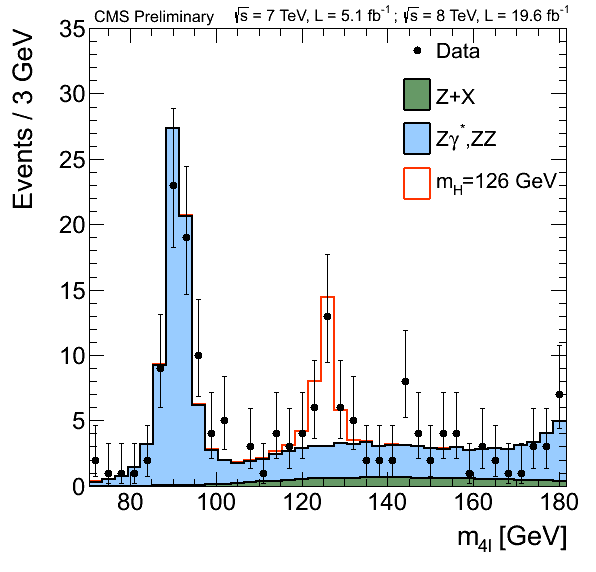
\includegraphics[height=.8\textheight, width=\linewidth,keepaspectratio]{\PhDthesisdir/plots_and_images/from_Hig13002TWiki/ZZMass_7Plus8TeV_70-180_3GeV.png}
\end{minipage}
\end{center}
\end{frame}
